\subsection{从存储工作负载图读取实际数据流}

存储工作负载图（Memory Workload Analysis）把左侧的逻辑存储空间与右侧的物理缓存层级联系起来。图\ref{l14:fig:memory-chart}中，左侧记录指令活动，中间记录向存储单元发出的请求，右侧箭头则显示 L1、L2 与设备内存之间的数据流量。不同位置的数字描述不同对象，不能因为都与“内存访问”有关就直接相互替代。

\begin{figure}[htbp]
\centering
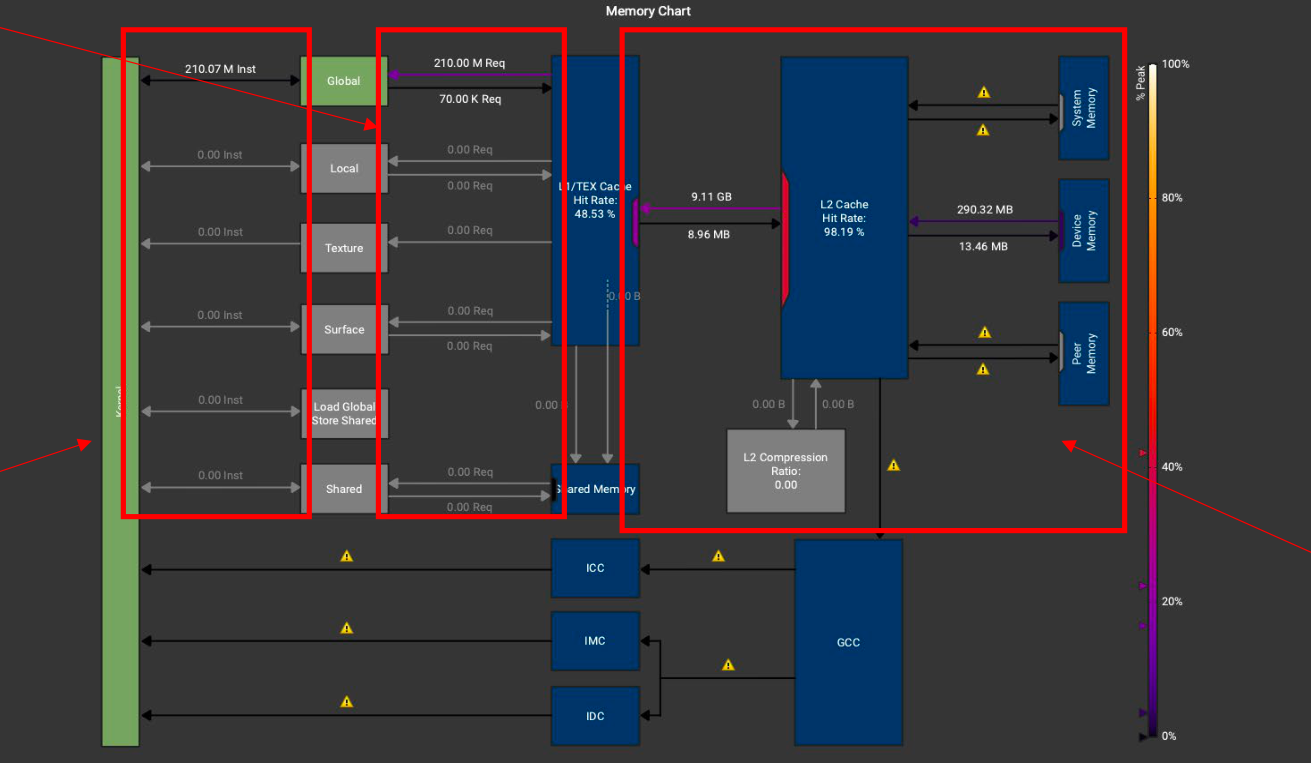
\includegraphics[width=0.87\textwidth]{memory_chart.png}
\caption{存储工作负载中的指令、请求与字节流量。读取可以在不同缓存层级得到满足，缓存命中与读写策略共同决定层级之间的流量。}
\label{l14:fig:memory-chart}
\end{figure}

\term{指令}{instruction}是实际执行的加载或存储操作；\term{请求}{request}是指令执行时向对应硬件单元提出的访问需求；\term{扇区}{sector}是缓存传输的计量粒度；\term{波前}{wavefront}表示硬件为了完成请求而进行的一轮服务。一个线程束的访存指令可以涉及多个地址、多个扇区或多个服务波前。报告中不少指令和请求指标以线程束为计数单位，而字节流量按实际传输计数，使用时还应核对单位。

在本讲的 L1／L2 访存分析中，一个扇区为 $32$ 字节。若同一请求的 $32$ 个线程分别读取 $4$ 字节，全部地址连续且与 $32$ 字节边界对齐，则共需 $128$ 字节，对应 $4$ 个扇区。地址分散时，硬件可能要搬入更多扇区，虽然线程最终使用的数据量没有增加。部分线程不活跃、广播或每线程访问宽度不同时，理想扇区数也会随之改变。

缓存命中率回答按指定统计单位计算的访问命中比例；本图中的 L1／L2 命中率按扇区统计，不能与请求命中率混用。吞吐率回答单位时间处理了多少数据或请求。高命中率与低延迟通常有利，但大量命中请求仍可能让片上入口、加载流水线或请求队列饱和。反过来，一次优化减少了请求数，却把访问顺序改变得更不利于复用，外层流量也可能上升。判断效果需要联合检查指令数、请求数、每请求扇区数、各层命中率和运行时间。

\subsection{全局访存合并与多余扇区}

\term{合并访存}{coalesced memory access}利用同一线程束各线程地址之间的空间关系，尽可能用较少的存储事务服务访问。表\ref{l14:tab:sectors}以 $32$ 个活跃线程、每线程读取一个单精度数为例，令 $j=0,\ldots,31$，$a_j$ 为第 $j$ 个线程的字节地址，并假定基地址为 $0$。各线程读取的数据互不重叠，实际需要的有用字节总数均为 $128$。

\begin{table}[htbp]
\centering\small
\caption{地址布局对所需扇区数量的影响}
\label{l14:tab:sectors}
\begin{tabularx}{\textwidth}{@{}p{30mm}p{25mm}p{28mm}Y@{}}
\toprule
地址形式 & 覆盖扇区数 & 扇区总字节 & 解释\\
\midrule
$a_j=4j$ & $4$ & $128$ & 连续且对齐，全部传输字节均有用\\
$a_j=4j+4$ & $5$ & $160$ & 连续访问跨过额外扇区边界\\
$a_j=8j$ & $8$ & $256$ & 每隔一个单精度元素读取，利用一半字节\\
$a_j=32j$ & $32$ & $1024$ & 每线程落入不同扇区，只使用其中 $4$ 字节\\
\bottomrule
\end{tabularx}
\end{table}

这个例子中的扇区利用比例可写为 $\eta_{\mathrm{sector}}=128/(32n_s)$，其中 $n_s$ 是实际覆盖的扇区数，四种布局分别得到 $100\%$、$80\%$、$50\%$ 和 $12.5\%$。这些是对应请求的传输效率；后续缓存命中可能再次改变设备内存实际流量，因此不能把该比例直接当成整机带宽效率。

多余扇区指标把某种理想访问需求与实际需要的扇区比较，用于定位可能存在的合并不足。它指出值得检查的代码位置，随后仍需结合每线程字节数、活跃线程数、对齐与请求类型解释。通常可以通过让相邻线程访问相邻元素、调整线程到输出的映射、修正行跨度或采用更合适的加载分工来改善。

对二维线程块，还应记住线程线性编号优先沿 $x$ 方向增长。例如 $16\times16$ 的线程块中，一个线程束跨越两行、每行 $16$ 个线程；是否高效取决于这两个半行分别覆盖多少扇区，以及行起点是否对齐。线程束跨两行本身不会必然导致浪费，必须代入实际地址分析。

\subsection{共享内存存储体与宽访问}

共享内存按\term{存储体}{bank}组织。在本讲使用的基本模型中，共有 $32$ 个存储体，连续的 $32$ 位字映射到连续存储体，每个存储体每周期提供一个 $32$ 位字的带宽。若字节地址为 $a$，则存储体编号为 $b(a)=\lfloor a/4\rfloor\bmod32$。访问无需按地址连续排列；只要同一次服务中的不同地址能分散到不同存储体，就可以并行服务。

\term{存储体冲突}{bank conflict}发生在同一服务阶段中，多个不同的 $32$ 位字映射到同一存储体，导致额外串行服务。多个线程读取同一个 $32$ 位字时，可以由一次读取及广播满足，包括该字内较窄的读取；这与读取同一存储体中的不同字有不同的代价。同地址并发写入则还涉及数据竞争，不能用读取广播来说明其正确性。

考虑完整线程束中的标量读取，每线程访问字索引 $w_j=w_0+sj$，其中步长 $s$ 是正整数，$32$ 个地址互不相同。存储体编号为 $(w_0+sj)\bmod32$。若两个线程间隔 $\Delta j$ 后落入同一存储体，就有 $s\Delta j\equiv0\pmod{32}$。令 $d=\gcd(s,32)$，最小正间隔是 $32/d$，所以访问覆盖 $32/d$ 个存储体，每个存储体需要服务 $d$ 个不同地址。在这个标量模型下，冲突程度就是 $d$。

因此，$s=1$ 访问全部 $32$ 个存储体，没有额外冲突；$s=2$ 只访问 $16$ 个存储体，形成两路冲突；$s=32$ 的 $32$ 个地址都落入同一存储体，形成 $32$ 路冲突；$s=33$ 又能覆盖全部存储体。二维共享数组宽度为 $32$ 时，沿列读取对应步长 $32$；将物理行宽填充到 $33$，就能让相邻行的同一列落入不同存储体。这个推导针对标量、互异地址；同地址广播和宽访问需要分别处理。

宽共享读取还要求区分每线程宽度和整个线程束的数据量。一条 \code{LDS.128} 指令中的 $128$ 表示每线程 $128$ 位，即 $16$ 字节，可以装入四个单精度数。若 $32$ 个线程读取互不相同的连续 $16$ 字节区域，总请求为 $512$ 字节；在常见的每轮 $128$ 字节服务模型下，需要四个理想波前。这些必需的波前属于访问宽度带来的工作量，不能仅因同一存储体在不同波前中重复出现就判为冲突。

共享访问的多余波前指标考察实际服务波前超过理想需求的部分，能够帮助定位冲突。向量化可能减少指令和请求数量，同时保留相同的传输字节数；若布局和对齐合适，它就能缓解指令队列压力。至于具体共享读取是否被编译为宽指令，以及额外波前是否下降，还需要结合机器指令与报告验证。
